\chapter{Homogeneous parallel ensembles: Bagging and random forests\label{Ch02}}
\section{Bagging: Bootstrap aggregating}
\textbf{Bagging}, short for \textbf{bootstrap aggregating}, was introduced by Leo Breiman in 1996. The
name refers to how bagging achieves ensemble diversity (through bootstrap sampling) and performs ensemble prediction (through model aggregating).
\begin{figure}
    \centering
    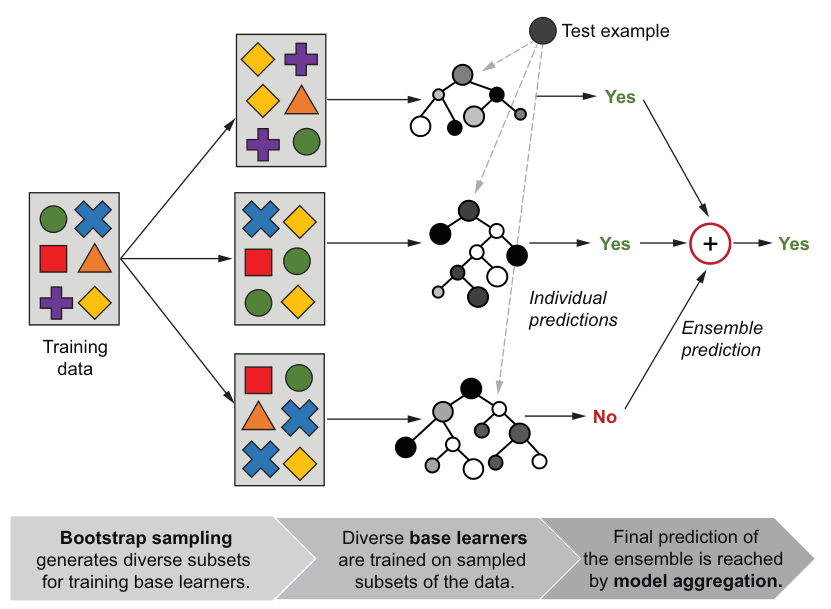
\includegraphics{../Figures/fig2-2.png}
    \caption{Bagging, illustrated. Bagging uses bootstrap sampling to generate similar but not exactly identical subsets (observe the replicates here) from a single data set. Models are trained on each of these subsets, resulting in similar but not exactly identical base estimators. Given a test example, the individual base-estimator predictions are aggregated into a final ensemble prediction. Also observe that training examples may repeat in the replicated subsets; this is a consequence of bootstrap sampling.}
\end{figure}

\figures{fig2-3}{
    Bootstrap sampling illustrated on a data set of six examples. By sampling with
    replacement, we can get a bootstrap sample size of six, containing only four unique objects
    but with repeats. Performing bootstrap sampling several times produces several replicates
    of the original data set—all of them with repeats.
}

\section{Random forests}
Random forests use a modified tree learning algorithm, which first randomly samples features before creating a decision node. The resulting tree is a \textbf{randomized decision tree}, which is a new type of base estimator.

Thus, random forests contain two types of randomization: (1) bootstrap sampling, similar to bagging; and (2) random feature sampling for learning randomized decision trees.

\figures{fig2-7}{Random forests use a modified tree learning algorithm, where a random feature subset is
    first chosen before the best splitting criterion for each decision node is identified. The unshaded columns
    represent features that have been left out; the lightly shaded columns represent available features from
    which the best feature is chosen, shown in the darkly shaded columns.}
\subsection{Feature importances}
One benefit of using random forests is that they also provide a natural mechanism for scoring features based on their importance. This means that we can rank features to identify the most important ones and drop less effective features, thus performing feature selection!

\section{More homogeneous parallel ensembles}
We’ve seen two important parallel homogeneous ensemble methods: bagging and
random forests. Let’s now explore a few variants that were developed for large data
sets (e.g., recommendation systems) or high-dimensional data (e.g., image or text
databases). These include bagging variants such as pasting, random subspaces and
random patches, and an extreme random forest variant called Extra Trees. All these
methods introduce randomization in different ways to ensure ensemble diversity.
\subsection{Pasting}
Bagging uses bootstrap sampling, or sampling with replacement. If, instead, we sample subsets for training \textbf{without replacement}, we have a variant of bagging known as \textbf{pasting}. \important{Pasting was designed for very large data sets, where sampling with replacement isn’t necessary}. Instead, because training full models on data sets of such scale is difficult, pasting aims to take small pieces of the data by sampling without replacement.
\begin{tcolorbox}[title=TIP]
    BaggingClassifier can easily be extended to perform pasting by setting bootstrap=False and making it subsample small subsets for training
    by setting max\_samples to a small fraction, say max\_samples=0.05.
\end{tcolorbox}

\subsection{Random subspaces and random patches}
\figures{fig2-9}{
    Bagging compared to random subspaces and random patches. The unshaded rows and
    columns represent training examples and features, respectively, that have been left out.
}

The key difference between random forests and bagging variants, such as random subspaces and random patches, is where the feature sampling occurs. Random forests
exclusively use randomized decision trees as base estimators. Specifically, \important{they perform feature sampling inside the tree learning algorithm} each time they grow the tree
with a decision node.

Random subspaces and random patches, on the other hand, aren’t restricted to tree
learning and can use any learning algorithm as a base estimator. They \important{randomly sample
    features once outside before calling the base-learning algorithm for each base estimator.}
\subsection{Extra Trees}
Extremely randomized trees take the idea of randomized decision trees to the
extreme by selecting not just the splitting variable from a random subset of features but also the splitting threshold!

Extremely randomized decision-tree learning also looks at a random subset of features to determine the best $f_k$. But to be even more efficient, it selects a random splitting threshold. Note that extremely randomized decision trees are yet another type of
base learner used for ensembling.

This extreme randomization is so effective, in fact, that we can construct an ensem-
ble of extremely randomized trees directly from the original data set without bootstrap
sampling! This means that we can construct an Extra Trees ensemble very efficiently.

\begin{tcolorbox}[title=TIP]
    In practice, Extra Trees ensembles are well suited for high-dimensional
    data sets with a large number of continuous features.
\end{tcolorbox}

scikit-learn provides an ExtraTreesClassifier that supports OOB estimation and
parallelization, much like BaggingClassifier and RandomForestClassifier.
Note that Extra Trees typically do not perform bootstrap sampling (bootstrap=False, by default), as we’re able to achieve base-estimator diversity through
extreme randomization.

\begin{tcolorbox}[title=CAUTION]
    scikit-learn provides two very similarly named classes: sklearn.
    tree.ExtraTreeClassifier
    and
    sklearn.ensemble.ExtraTreesClassifier. The tree.ExtraTreeClassifier class is a base-learning algorithm and should be used for learning individual models or as a base estimator
    with ensemble methods. ensemble.ExtraTreesClassifier is the ensemble method discussed in this section. The difference is in the singular usage of
    “Extra Tree” (ExtraTreeClassifier is the base learner) versus the plural
    usage “Extra Trees” (ExtraTreesClassifier is the ensemble method).
\end{tcolorbox}

\section{Case study: Breast cancer diagnosis}
\subsection{Bagging, random forests, and Extra Trees}
\subsubsection*{ENSEMBLE SIZE VS. ENSEMBLE PERFORMANCE}
\subsubsection*{BASE LEARNER COMPLEXITY VS. ENSEMBLE PERFORMANCE}
One key consideration in determining the depth of the base decision trees is computational efficiency. Training deeper and deeper trees will take more and more time
without producing a significant improvement in predictive performance.


\begin{tcolorbox}[title=CAUTION]
    Note that feature importances will often change between runs
    owing to randomization during tree construction. Note also that if two features are highly correlated, random forests will often distribute the feature
    importance between them, leading to their overall weights appearing smaller
    than they actually are.
\end{tcolorbox}

\section{Summary}
\begin{itemize}

    \item Parallel homogeneous ensembles promote ensemble diversity through randomization: random sampling of training examples and of features, or even introducing randomization in the base-learning algorithm.
    \item Bagging is a simple ensemble method that relies on (1) bootstrap sampling (or
          sampling with replacement) to generate diverse replicates of the data set and
          training diverse models, and (2) model aggregation to produce an ensemble
          prediction from a set of individual base learner predictions.
    \item Bagging and its variants work best with any unstable estimators (unpruned decision trees, support vector machines [SVMs], deep neural networks, etc.), which
          are models of higher complexity and/or nonlinearity.
    \item Random forest refers to a variant of bagging specifically designed to use randomized decision trees as base learners. Increasing randomness increases
          ensemble diversity considerably, allowing the ensemble to decrease the variability and smooth out predictions.
    \item Pasting, a variant of bagging, samples training examples without replacement
          and can be effective on data sets with a very large number of training examples.
    \item Other variants of bagging, such as random subspaces (sampling features) and
          random patches (sampling both features and training examples), can be effective on data sets with high dimensionality.
    \item Extra Trees is another bagging-like ensemble method that is specifically
          designed to use extremely randomized trees as base learners. However, \important{Extra
              Trees doesn’t use bootstrap sampling} as additional randomization helps in generating ensemble diversity.
    \item Random forests provide feature importances to rank the most important features from a predictive standpoint.
\end{itemize}